\documentclass[a4paper]{article}
\usepackage{color}
\usepackage{tikz}
\usepackage{ntheorem}
\usepackage{caption}
\usepackage{subcaption}
\theoremseparator{:}
\newtheorem{hyp}{Hypothesis}
\usetikzlibrary{shapes,decorations,arrows,calc,arrows.meta,fit,positioning}
\tikzset{
    -Latex,auto,node distance =1 cm and 1 cm,semithick,
    state/.style ={ellipse, draw, minimum width = 0.7 cm},
    point/.style = {circle, draw, inner sep=0.04cm,fill,node contents={}},
    bidirected/.style={Latex-Latex,dashed},
    el/.style = {inner sep=2pt, align=left, sloped}
}
\begin{document}
\section{Data Prep, EDA, and Theory development}
\subsection{Varaible Selection \& Explanation}


\begin{figure}
     \centering
     \begin{subfigure}[b]{0.45\textwidth}
         \centering
         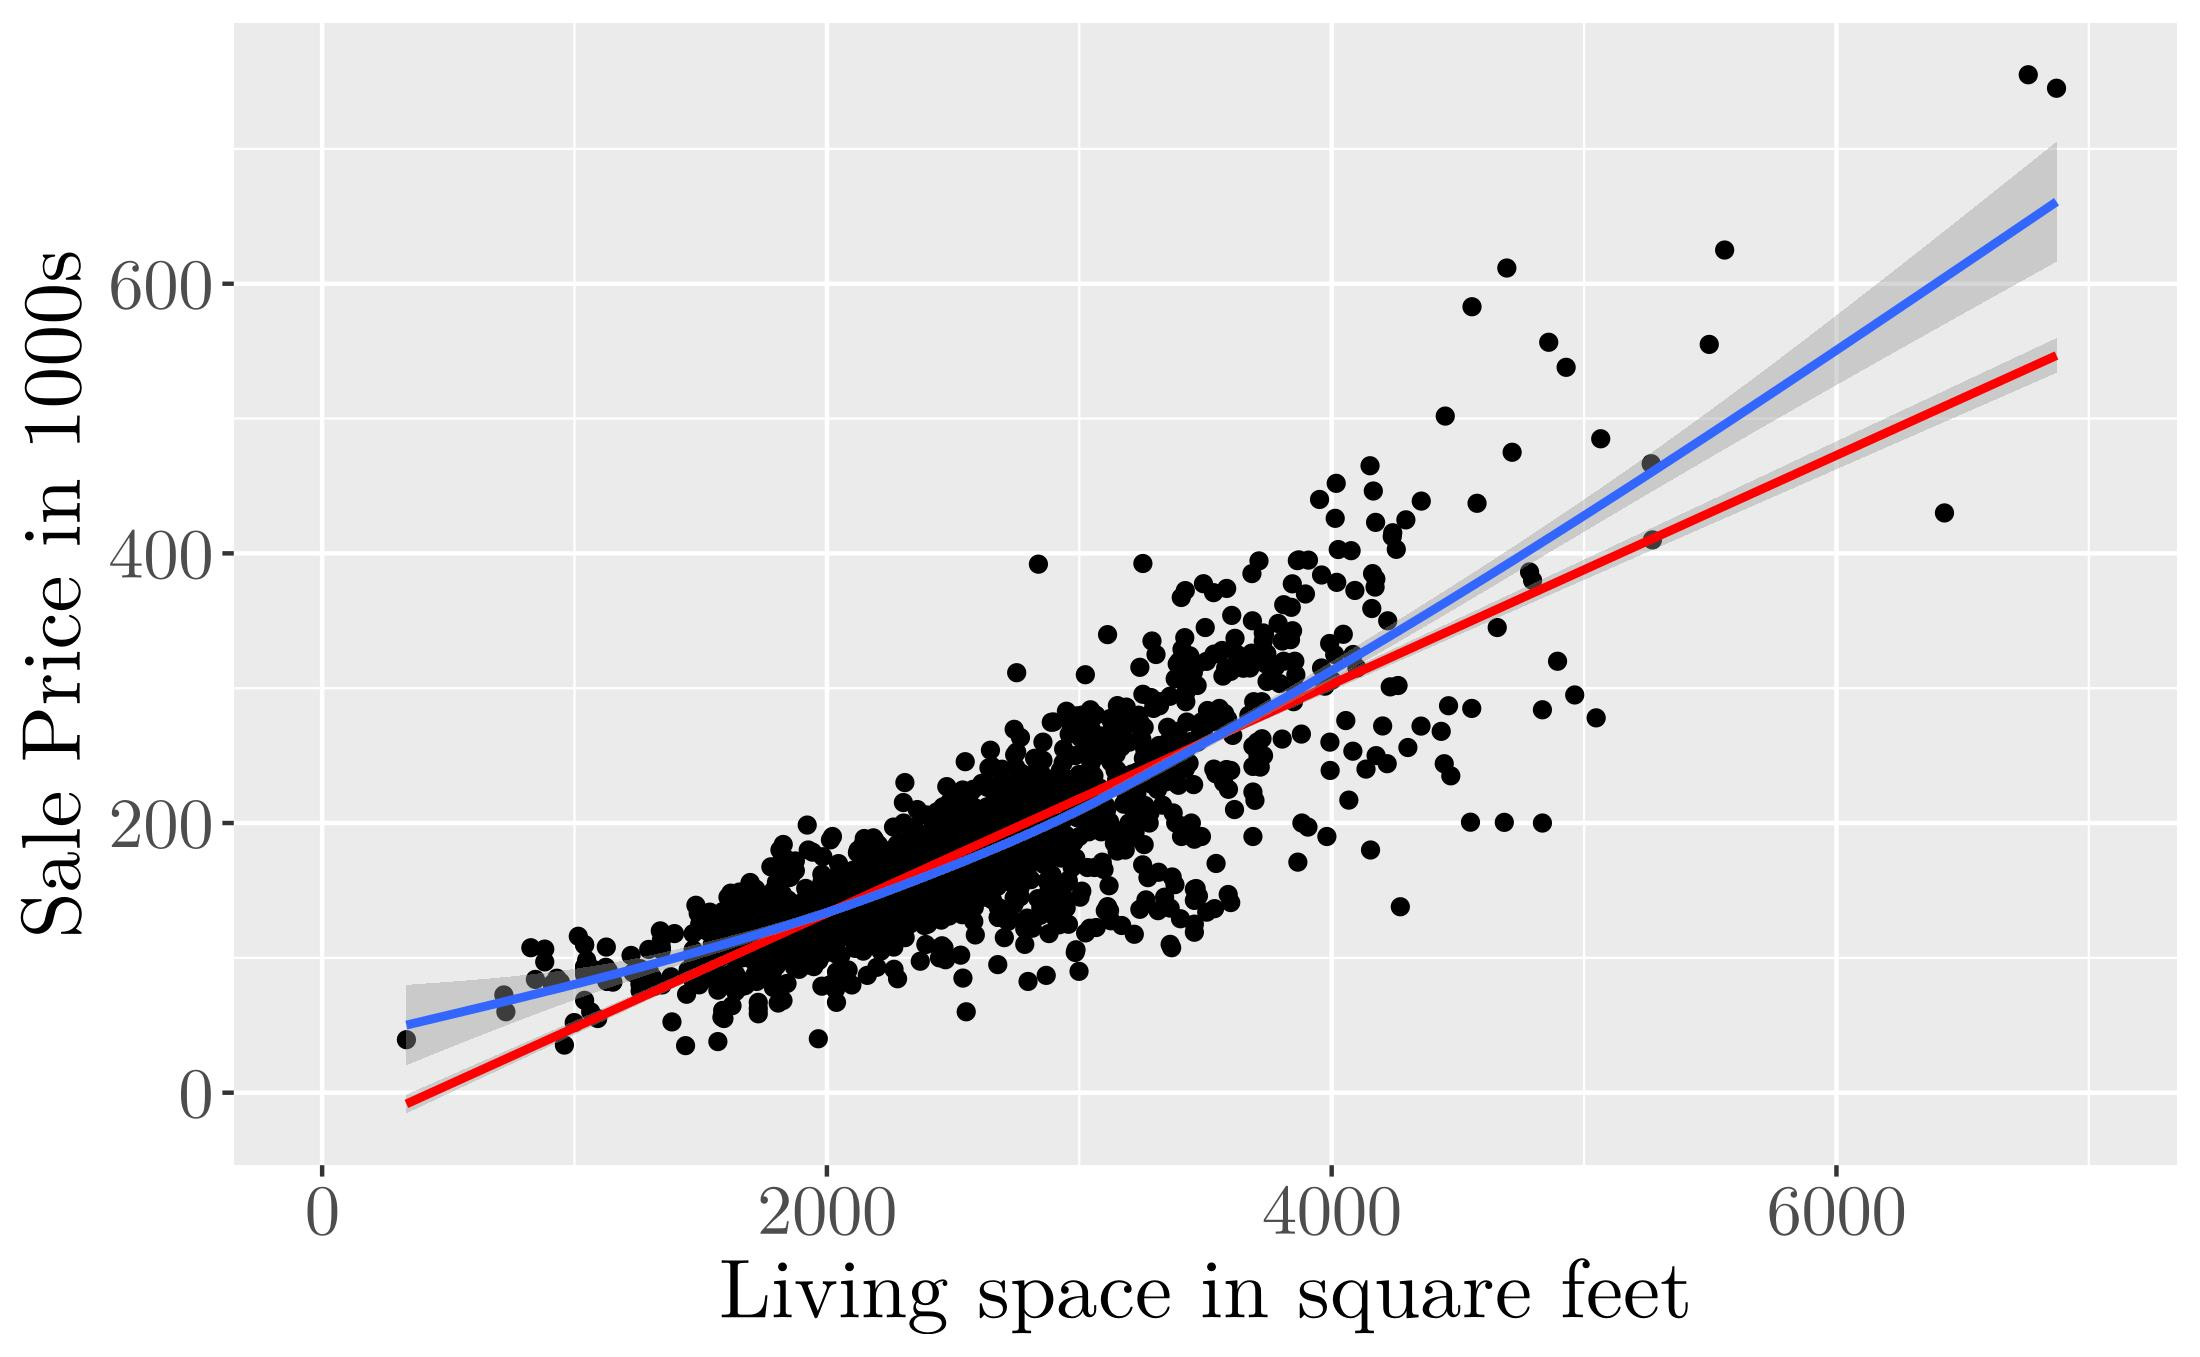
\includegraphics[scale=0.3]{"/home/angelo/Documents/Uni/Courses/Advanced Statistics and programming/Assignments/assignment1/Code/h1.jpg"}
         \caption{Positive association of total Living Space \& Sale Price \& optimal line}
         \label{fig:y equals x}
     \end{subfigure}
     \hfill
     \begin{subfigure}[b]{0.45\textwidth}
         \centering
         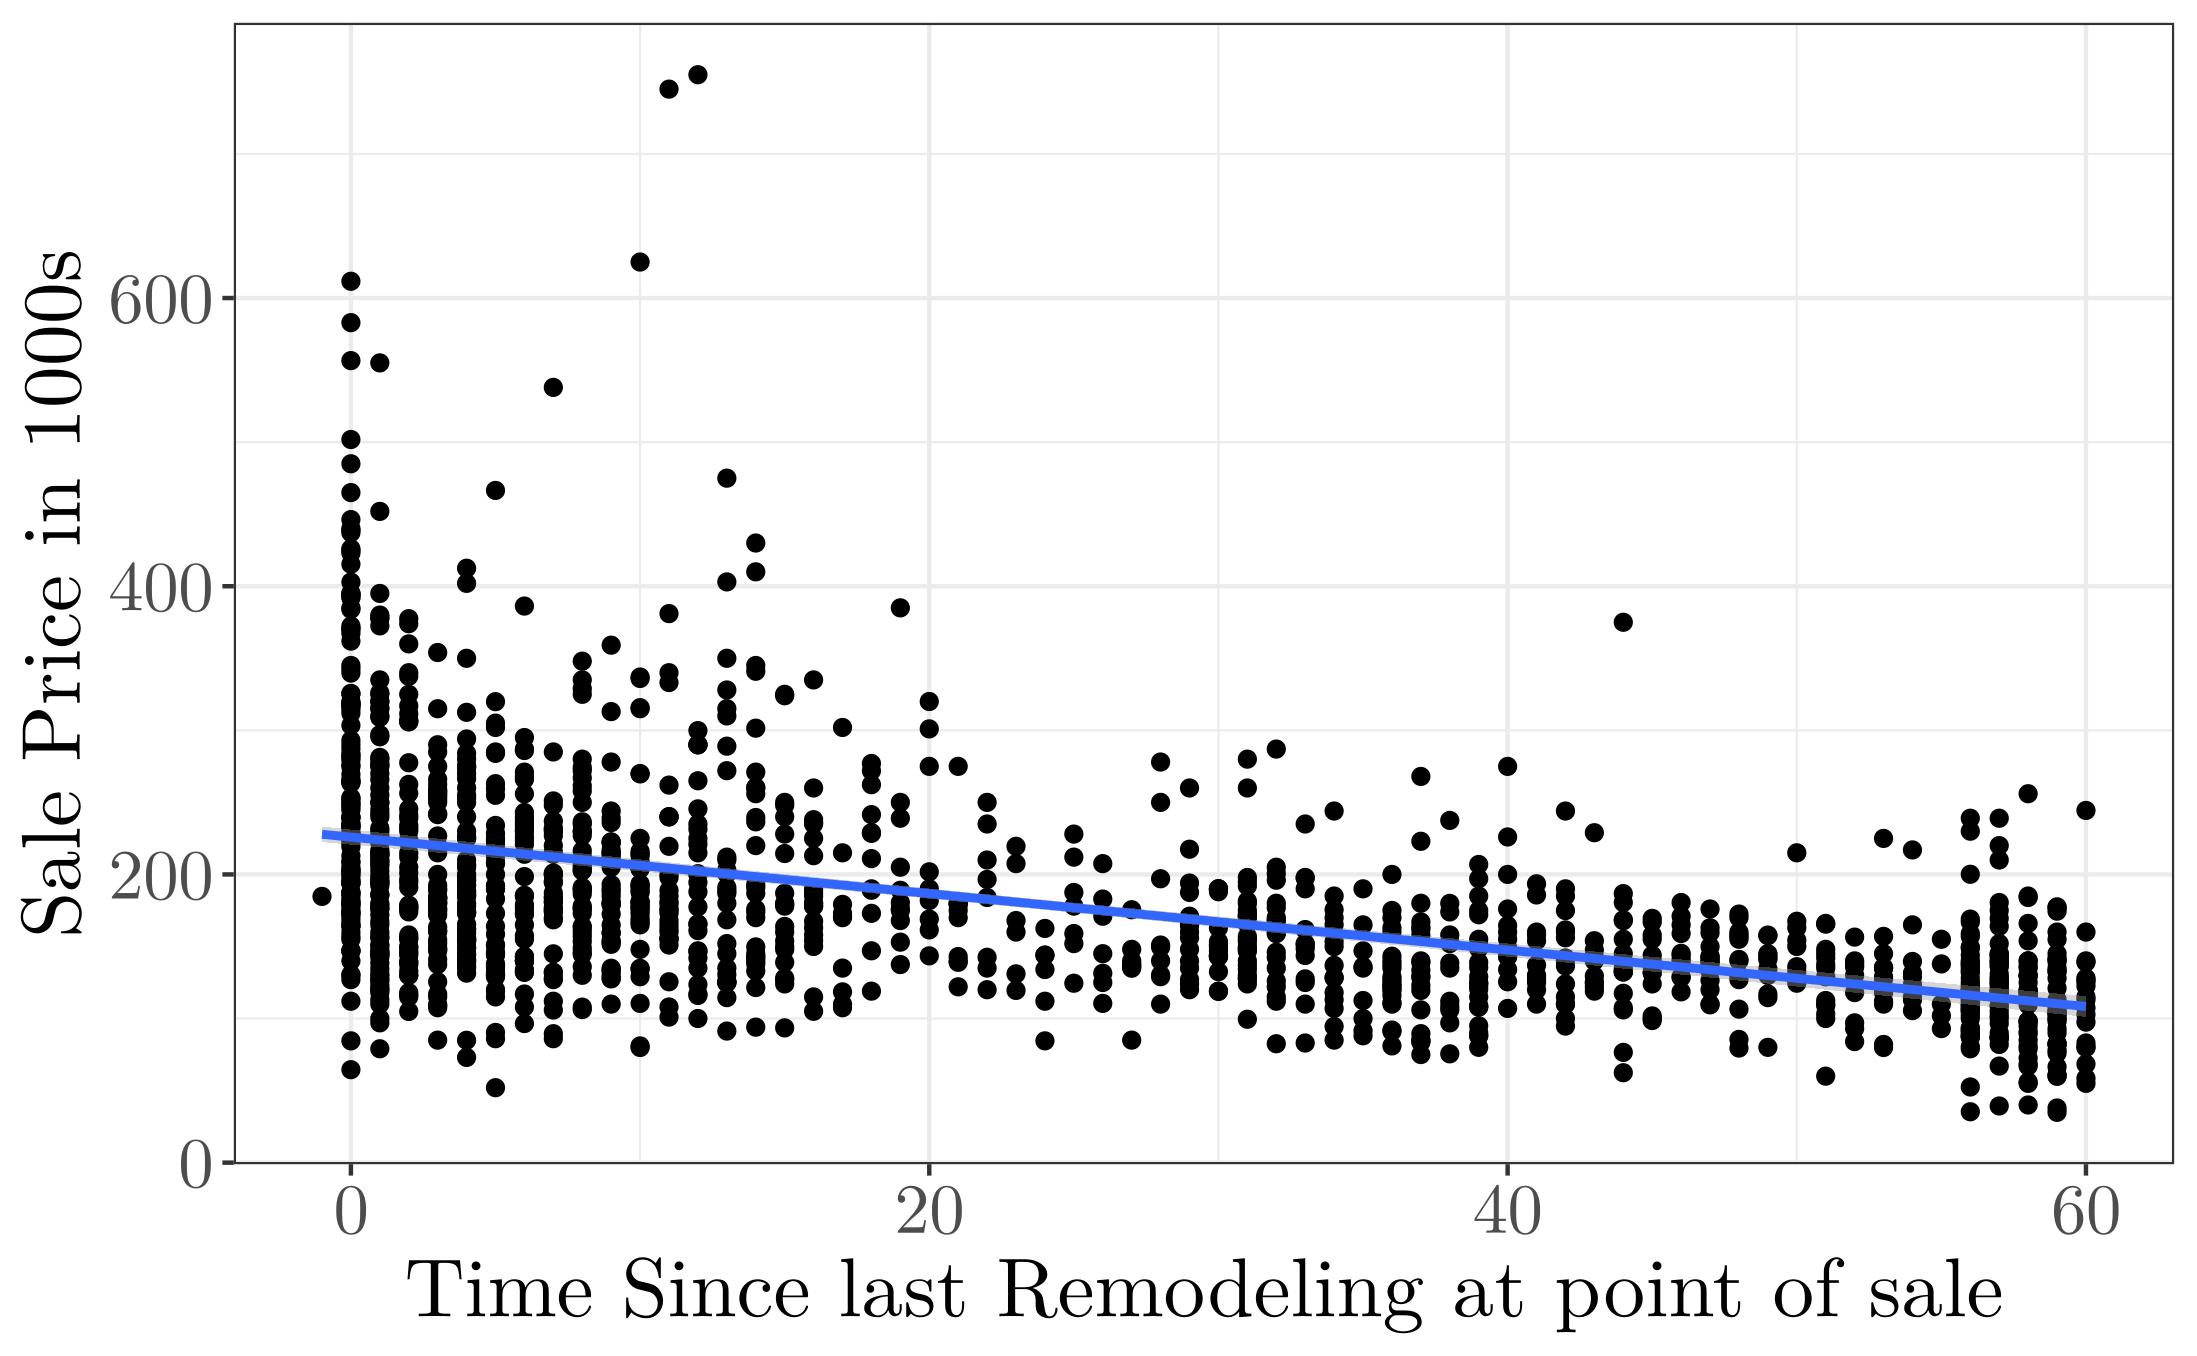
\includegraphics[scale=0.30]{"/home/angelo/Documents/Uni/Courses/Advanced Statistics and programming/Assignments/assignment1/Code/h3.jpg"}
         \caption{Positive association of total Living Space \& Sale Price}
         \label{fig:three sin x}
     \end{subfigure}
     \hfill
     \begin{subfigure}[b]{0.45\textwidth}
         \centering
         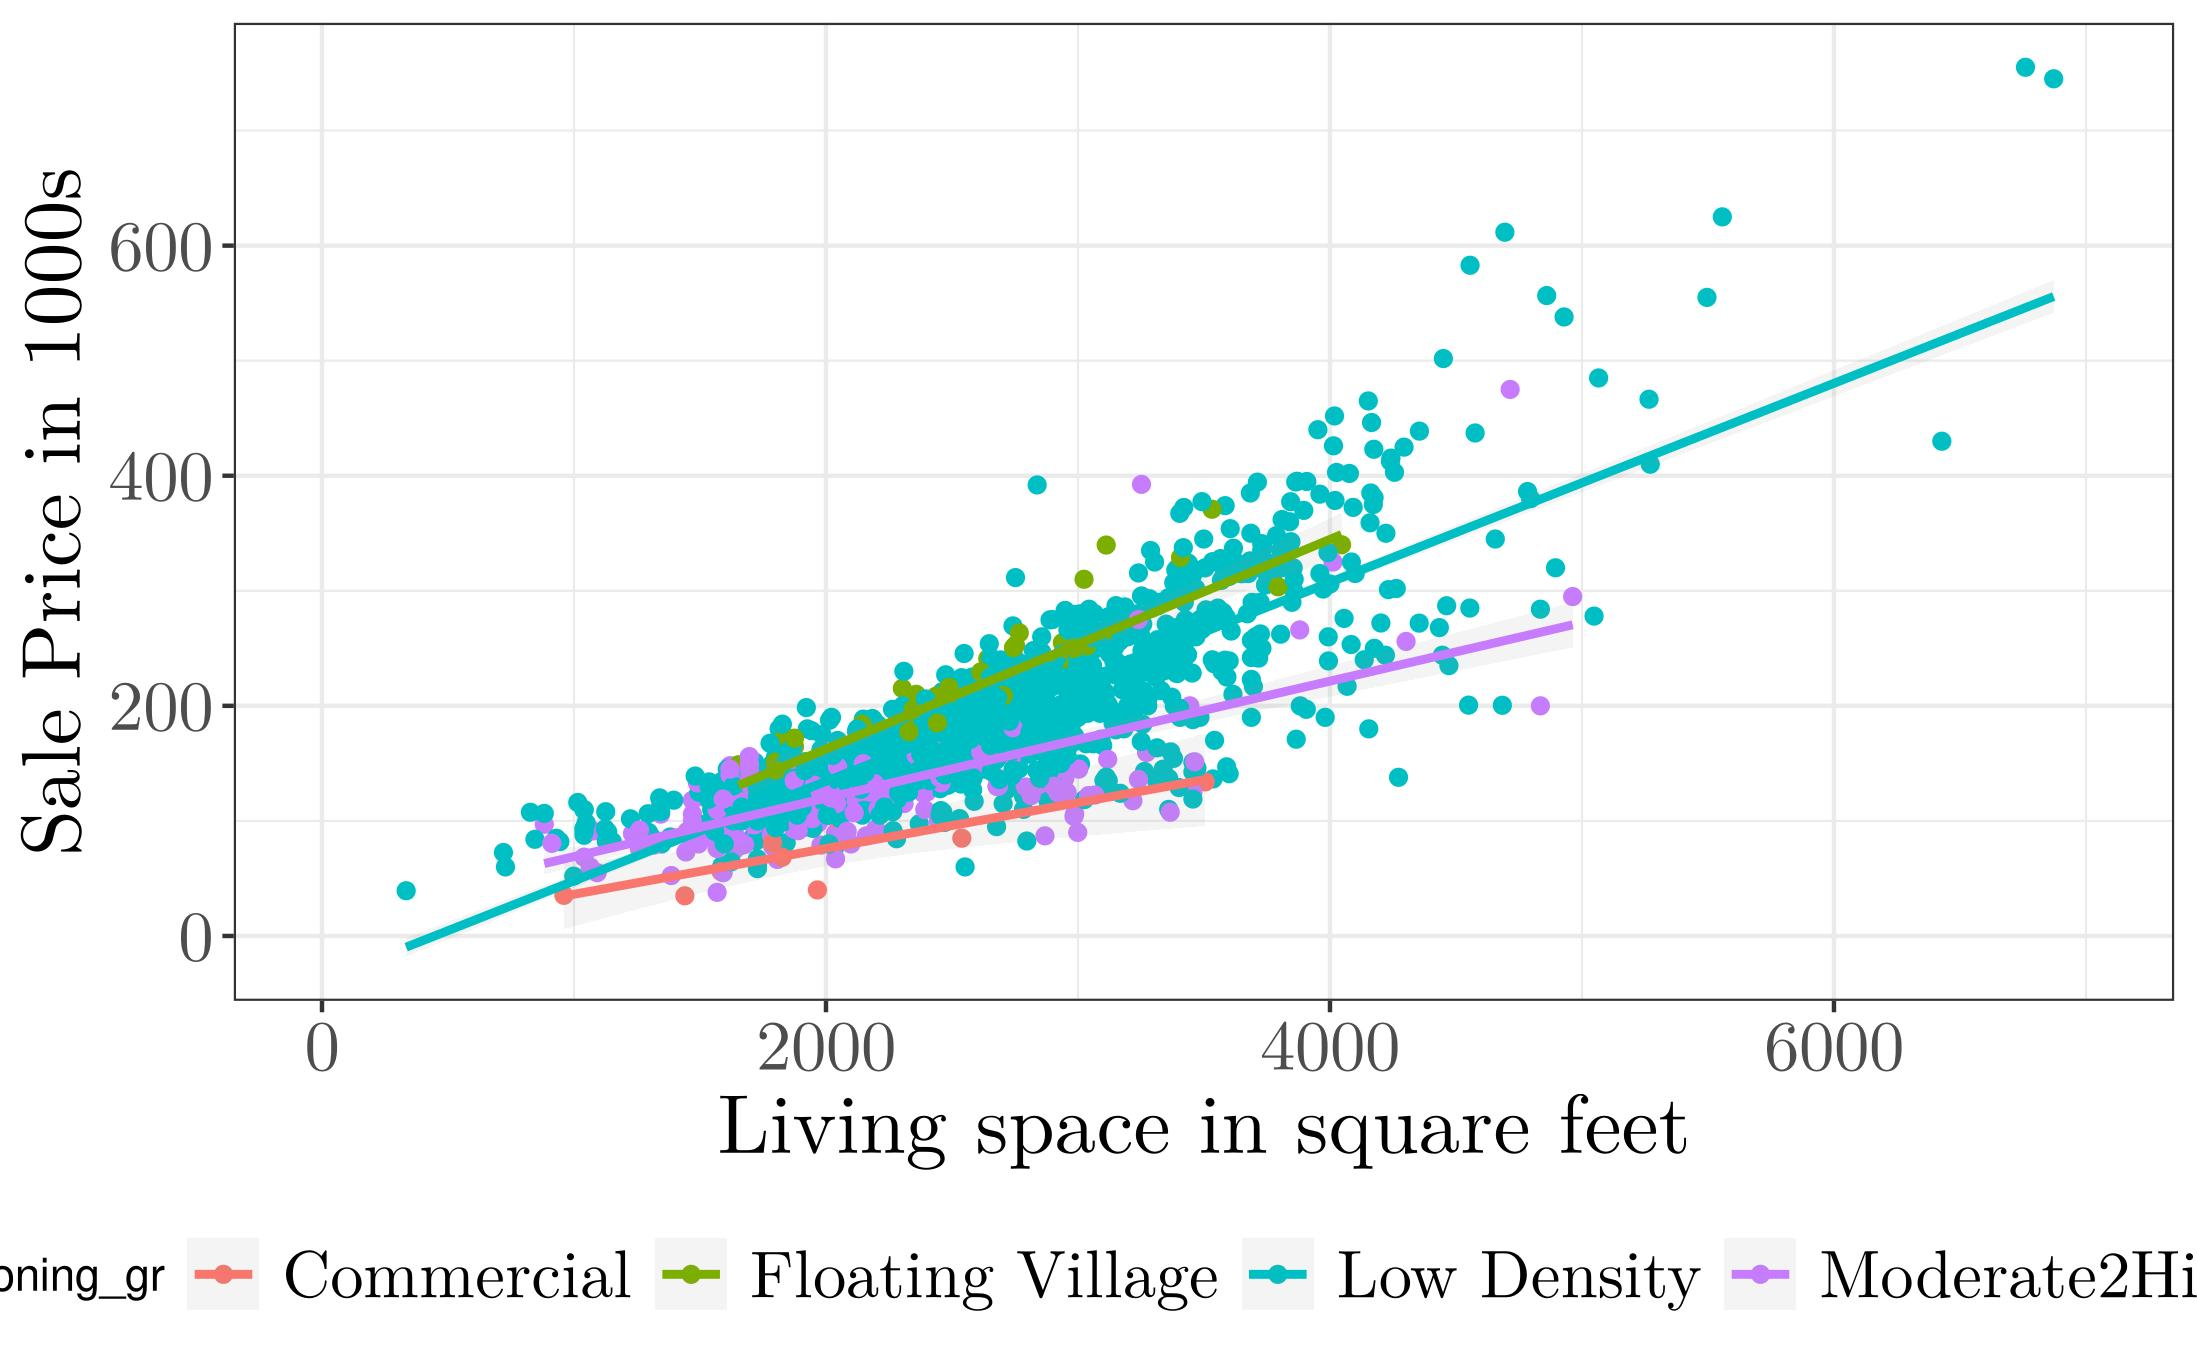
\includegraphics[scale=0.325]{"/home/angelo/Documents/Uni/Courses/Advanced Statistics and programming/Assignments/assignment1/Code/h2.2.jpg"}
         \caption{Positive association of total Living Space \& Sale Price}
         \label{fig:five over x}
     \end{subfigure}
        \caption{Three Hypothesis Graphs displaying their repective association with the outcome variable}
        \label{fig:three graphs}
\end{figure}





















\begin{center}
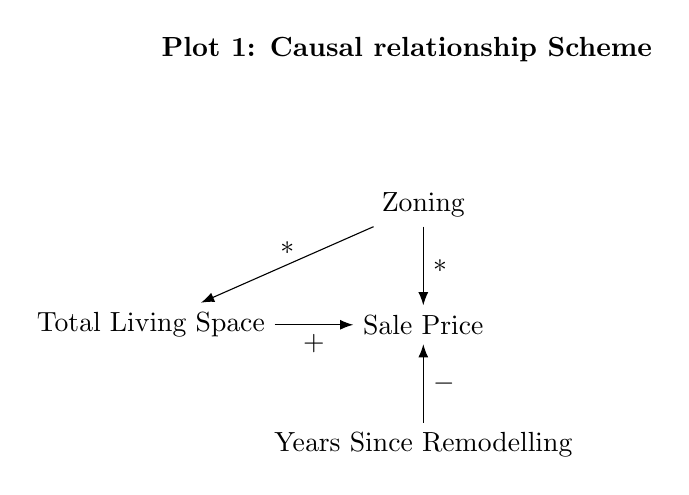
\begin{tikzpicture}
	\centering
 	\node at (3.25,3.5) {\textbf{Plot 1: Causal relationship Scheme}};
    \node (1) at (0,0) {Total Living Space};
	\node (2) [right = of 1] {Sale Price};
	\node (3) [above = of 2] {Zoning};
	\node (4) [below = of 2] {Years Since Remodelling};

	\path (1) edge node[below] {$+$} (2);
	\path (3) edge node[right] {$*$} (2);
	\path (3) edge node[above] {$*$} (1);
	\path (4) edge node[right] {$-$} (2);
	
\end{tikzpicture}
\end{center}




\end{document}